\section{Promela-C-Integration}
\begin{figure}
  \centering
  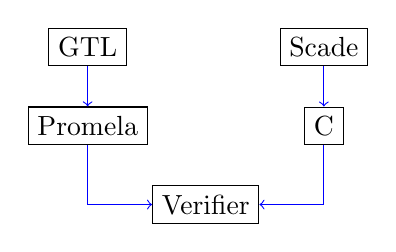
\begin{tikzpicture}
    \node[draw] (gtl) at (0,2) {GTL};
    \node[draw] (scade) at (3,2) {Scade};
    \node[draw] (promela) at (0,1) {Promela};
    \node[draw] (c) at (3,1) {C};
    \node[draw] (verifier) at (1.5,0) {Verifier};
    \draw[->,blue] (gtl) -- (promela);
    \draw[->,blue] (scade) -- (c);
    \draw[->,blue] (promela) |- (verifier);
    \draw[->,blue] (c) |- (verifier);
  \end{tikzpicture}
  \caption{Simulation durch C-Integration von Promela}
\end{figure}

Diese Übersetzungsmethode führt keine Optimierungen oder Abstraktionen durch, sondern simuliert das Modell exakt so, wie durch die Spezifikation angegeben.
Die Kontrakte für die synchronen Komponenten werden also ignoriert.
Um die Komponenten zu simulieren reichen die Informationen in der GTL-Spezifikation nicht aus, denn die Modell sind hier nur als Referenzen vorhanden.
Die eigentliche Implementierung findet in den synchronen Formalismen statt, also in dieser Arbeit in SCADE.
Die SCADE-Komponenten müssen also nach Promela übersetzt werden, damit das Gesamtmodell simuliert und verifiziert werden kann.
Eine direkte Übersetzung ist zwar prinzipiell möglich, aber aufgrund der Mächtigkeit der SCADE Sprache mit sehr viel Aufwand verbunden.
Einfacher ist es, die von SCADE angebotene C-Übersetzung zu verwenden und den generierten C-Code in Promela einzubinden, was SPIN seit Version 4 erlaubt.

Zunächst wird jede synchrone Komponente mit Hilfe des SCADE-Compilers nach C übersetzt.
Da der Übersetzungsprozess für jede Komponente einzeln durchgeführt werden muss, muss darauf geachtet werden, dass die Modelle keine Namenskonflikte aufweisen oder die gleichen Sub-Komponenten enthalten\cite{scade_c_integration}.

Der Compiler generiert nun für jede Komponente zwei Datenstrukturen, die erste enthält die Eingabevariablen und erhält das Namensprefix "`inC\_"', die zweite enthält die Ausgabevariablen sowie den internen Zustand der Komponente und ist mit dem Prefix "`outC\_"' versehen.
Außerdem werden zwei Funktionen erstellt:
Die erste initialisiert den internen Zustand der Komponente und hat das Suffix "`\_reset"', die zweite führt einen einzelnen Berechnungsschritt der Komponente durch und ist genau wie die Komponente benannt.

%Jede synchrone Komponente wird nun durch einen Promela-Prozess repräsentiert, der zunächst die Datenstrukturen initialisiert und dann in jedem Schritt die Eingabevariablen in die C-Datenstruktur kopiert, die Schrittfunktion aufruft und die Ergebnisse in die Ausgabevariablen schreibt.
Die Übersetzung geht nun wie folgt vor:
Zunächst wird für jeden Prozess eine Instanz der Zustands-Datenstruktur zum globalen Zustandsvektor hinzugefügt.
Dies geschieht über die Verwendung des "`c\_state"'-Konstruktes in Promela.
Eine Komponente "`Engine"' würde beispielsweise den folgenden Code generieren:
\begin{lstlisting}[language=promela]
c_state "outC_Engine Engine_state" "Global"
\end{lstlisting}
Dies fügt dem Zustandsvektor die Variable "`Engine\_state"' hinzu.
Das Schlüsselwort "`Global"' führt dazu, dass auf die Variable von jedem Prozess aus zugegriffen werden kann.

Die Eingabe-Datenstruktur der Komponenten ist für den Zustand des Gesamtsystems nicht entscheidend, sondern wird nur benötigt, um die Eingabesignale der Komponente vor dem Berechnungsschritt zu sammeln.
Deswegen ist es ausreichend, die Struktur mit dem "`c\_decl"'-Konstrukt zu deklarieren:
\begin{lstlisting}[language=promela]
c_decl {
  inC_Engine Engine_input;
}
\end{lstlisting}

Zur korrekten Simulation der synchronen Komponente müssen nun folgende Dinge geschehen:
\begin{enumerate}
\item Am Anfang der Simulation muss die Zustands-Datenstruktur der Komponente initialisiert werden.
  Hierfür generiert der Code-Generator eine "`reset"' Funktion:
  \begin{lstlisting}[language=promela]
c_code {
  Engine_reset(&now.Engine_state);
}
  \end{lstlisting}
\item In jedem Berechnungsschritt müssen die Eingaben für die Komponente aus den Aus\-ga\-be-Da\-ten\-struk\-tu\-ren der verbundenen Komponenten kopiert werden.
  \begin{lstlisting}[language=promela]
c_code {
  Engine_input.power = now.Power_state.on;
  Engine_input.mode = now.SpeedRegulator_state.output;
}
  \end{lstlisting}
\item Die generierte Schrittfunktion der Komponente muss aufgerufen werden.
  \begin{lstlisting}[language=promela]
c_code {
  Engine(&Engine_input,&now.Engine_state);
}
  \end{lstlisting}
\end{enumerate}
Die gesamte Übersetzung des vorgestellten Modells sieht also so aus:
\begin{lstlisting}[language=promela]
c_code {
  \#include "Engine.h"
}

c_state "outC_Engine Engine_state" "Global"

c_decl {
  inC_Engine Engine_input;
}

proctype Power { ... }
proctype SpeedRegulator { ... }

proctype Engine {
  c_code {
    Engine_reset(&now.Engine_state);
  };
  do
  :: c_code {
       Engine(&Engine_input,&now.Engine_state);
     }
  od
}
\end{lstlisting}
Problematisch bei der C-Übersetzung ist allerdings zu sehen, dass der übersetzte Code alle Ausgabevariablen der Komponente in den Zustandsraum der Komponente übernimmt, obwohl sie eventuell gar nicht für den Folgezustand der Komponente entscheidend sind.
Das kann dazu führen, dass die Verifikation mit der C-Übersetzung mehr Zustände generiert als es eine äquivalente, auf direkter Übersetzung basierende Übersetzung tun würde.
Das Problem kann für die C-Übersetzung nicht umgangen werden, da die Information, ob eine Ausgabevariable für den nächsten Zustand verantwortlich ist, tiefergehende Analysen des SCADE Modells erfordern würden, die auf einer quasi-Übersetzung des SCADE-Codes nach Promela gleich käme.